%%%%%%%%%%%%%%%%%%%%%%%% main.tex %%%%%%%%%%%%%%%%%%%%%%%%%%%%%
% Seminarska naloga: Modeliranje krožne topologije P2P v orodju OMNeT++
%%%%%%%%%%%%%%%%%%%%%%%%%%%%% Springer %%%%%%%%%%%%%%%%%%%%%%%%%%

\documentclass[graybox, envcountchap]{svmult}

\usepackage{mathptmx}
\usepackage{helvet}
\usepackage{courier}
\usepackage{makeidx}
\usepackage{graphicx}
\usepackage{hyperref}
\usepackage{epsfig}
\graphicspath{{./img/}}
\usepackage{multicol}
\usepackage[bottom]{footmisc}
\usepackage{epstopdf}
\usepackage{amsmath}
\usepackage{physics}
\usepackage{listings}
\usepackage{color}
\usepackage{amssymb}
\usepackage{xurl}
\usepackage{subcaption}
\usepackage{multirow}
\usepackage{tabularx}
\usepackage{caption}
\usepackage{float}
\usepackage{tikz}
\usepackage{pgfplots}
\pgfplotsset{compat=1.17}
\usepackage[utf8]{inputenc}
\usepackage[slovene]{babel}

\definecolor{codegreen}{rgb}{0,0.6,0}
\definecolor{codegray}{rgb}{0.5,0.5,0.5}
\definecolor{codepurple}{rgb}{0.58,0,0.82}
\definecolor{backcolour}{rgb}{0.95,0.95,0.92}

\lstdefinestyle{mystyle}{
    backgroundcolor=\color{backcolour},
    commentstyle=\color{codegreen},
    keywordstyle=\color{blue},
    numberstyle=\tiny\color{codegray},
    stringstyle=\color{codepurple},
    basicstyle=\ttfamily\footnotesize,
    breakatwhitespace=false,
    breaklines=true,
    captionpos=b,
    keepspaces=true,
    numbers=left,
    numbersep=5pt,
    showspaces=false,
    showstringspaces=false,
    showtabs=false,
    tabsize=2
}
\lstset{style=mystyle}

\makeindex

\begin{document}

\title{Modeliranje krožne topologije P2P v orodju OMNeT++}
\author{Stefan Jakjoski, Branko Raičković, Nik Janoš in Tadej Pariš}
\maketitle

\abstract*{V tem seminarju predstavljamo modeliranje in simulacijo krožne (ring) topologije omrežja v orodju OMNeT++. Analiziramo vpliv različnih parametrov na zmogljivost omrežja, s posebnim poudarkom na povprečnem času potovanja paketa od izvornega do ponornega vozlišča. Implementirali smo enostavno P2P krožno omrežje s 7 vozlišči in analizirali delovanje pri različnih obremenitvah (1 Mbps, 30 Mbps, 150 Mbps in 500 Mbps). Rezultati kažejo, da ima hitrost prenosa podatkov ključen vpliv na zakasnitev in zasedenost čakalnih vrst.}

\abstract{V tem seminarju predstavljamo modeliranje in simulacijo krožne (ring) topologije omrežja v orodju OMNeT++. Analiziramo vpliv različnih parametrov na zmogljivost omrežja, s posebnim poudarkom na povprečnem času potovanja paketa od izvornega do ponornega vozlišča. Implementirali smo enostavno P2P krožno omrežje s 7 vozlišči in analizirali delovanje pri različnih obremenitvah (1 Mbps, 30 Mbps, 150 Mbps in 500 Mbps). Rezultati kažejo, da ima hitrost prenosa podatkov ključen vpliv na zakasnitev in zasedenost čakalnih vrst.}

%%%%%%%%%%%%%%%%%%%%%%%%%%%%%%%%%%%%%%%%%%%%%%%%%%%%%%%%%%%%%%%%%%%%%%%%%%%%%%%
\section{Uvod in motivacija}
\label{sec:uvod}

Omrežne topologije predstavljajo temeljni koncept pri načrtovanju računalniških omrežij. Izbira pravilne topologije je ključnega pomena za zagotavljanje učinkovitega prenosa podatkov, minimizacijo zakasnitev in obvladovanje prometnih nasičenj.

V tem seminarju obravnavamo štiri najpogostejše omrežne topologije:

\begin{enumerate}
    \item \textbf{Zvezdasta topologija (Star)} -- V omrežju z zvezdasto topologijo je vsaka naprava povezana na skupno centralno vozlišče (hub). Ločimo aktivno in pasivno zvezdasto topologijo. Pri aktivni centralno vozlišče pošlje prejeto sporočilo napravam v omrežju, pri pasivni pa centralno vozlišče služi le kot povezava.
    
    \subsubsection*{Prednosti}
    \begin{itemize}
        \item Odpornost do napak
        \item Eliminira trke paketov
        \item Cenovno ugodno: vsaka naprava potrebuje le ena vrata za komunikacijo
        \item Raztegljivo: dodajanje naprave ne spremeni strukture obstoječega omrežja
        \item Enostavna diagnoza napak
    \end{itemize}
    
    \subsubsection*{Slabosti}
    \begin{itemize}
        \item Centralno vozlišče je točka odpovedi
        \item Zmogljivost odvisna od centralnega vozlišča
    \end{itemize}
    
    \item \textbf{Mrežna topologija (Mesh)} -- V omrežju z mesh topologijo je vsaka naprava povezana direktno z vsako drugo napravo. Tako omrežje je torej decentralizirano.
    
    \subsubsection*{Prednosti}
    \begin{itemize}
        \item Več možnih poti omogoča boljšo odpornost do napak: če povezava odpove, uberemo drugo pot
        \item Raztegljivo (scalable) omrežje: dodajanje naprave ne spremeni strukture obstoječega omrežja
        \item Učinkovit prenos podatkov: ne potujejo skozi centralno vozlišče
    \end{itemize}
    
    \subsubsection*{Slabosti}
    \begin{itemize}
        \item Kompleksna izdelava in vzdrževanje: vsaka naprava je povezana z vsako
        \item Visoka cena
        \item Možnost redundantnih povezav
    \end{itemize}
    
    \item \textbf{Krožna topologija (Ring)} -- Krožna point-to-point topologija (ali topologija obroča) opisuje omrežje, kjer je vsaka naprava povezana z natanko dvema drugima napravama v zaprti zanki. Krožne topologije omogočajo krožni prenos podatkov med $n$ vozlišči. Podatkovni paketi potujejo v eno smer in prehajajo skozi vsako vozlišče v obroču, dokler ne dosežejo cilja.
    
    V krožnih topologijah lahko podatke hkrati prenaša le eno vozlišče. To se nadzoruje z žetonom, ki kroži po omrežju in omogoča posameznemu vozlišču prenos podatkov. Vozlišče ne sme prenašati podatkov brez posedovanja žetona.
    
    \subsubsection*{Prednosti}
    \begin{itemize}
        \item Naenkrat lahko prenaša le eno vozlišče, kar zmanjšuje trke paketov
        \item Implementacija je pogosto preprosta; kompleksnost dodajanja več vozlišč se linearno skalira, za razliko od kvadratnega skaliranja mrežaste topologije
    \end{itemize}
    
    \subsubsection*{Slabosti}
    \begin{itemize}
        \item Če eno vozlišče odpove, se celotno omrežje izklopi
        \item Zmogljivost omrežja je enostavno preobremeniti
    \end{itemize}
    
    \item \textbf{Spine Leaf topologija} -- Je topologija, sestavljena iz dveh slojev stikal: leaf in spine. Uporabljena je v glavnem v podatkovnih centrih, kjer imamo opravka z velikim številom naprav. Je alternativa tradicionalni troslojni arhitekturi. Leaf so stikala, ki prejemajo podatke, spine pa so stikala, ki leaf sloj povezujejo v mrežasto topologijo.
    
    \subsubsection*{Prednosti}
    \begin{itemize}
        \item Redundanca stikal
        \item Raztegljivost
        \item Nizka latenca v primerjavi s tradicionalno
    \end{itemize}
    
    \subsubsection*{Slabosti}
    \begin{itemize}
        \item Potrebujemo več stikal
        \item Za veliko uporab prekompleksna topologija
    \end{itemize}
\end{enumerate}

V tem delu podrobno analiziramo \textbf{krožno topologijo P2P} in jo implementiramo v orodju OMNeT++. Krožna topologija je posebej primerna za analizo prometnih nasičenj, saj ima deterministično pot prenosa -- vsak paket potuje od izvornega do ciljnega vozlišča po krožni poti \cite{omnetpp}.

%%%%%%%%%%%%%%%%%%%%%%%%%%%%%%%%%%%%%%%%%%%%%%%%%%%%%%%%%%%%%%%%%%%%%%%%%%%%%%%
\section{Opis protokola}
\label{sec:protokol}

V implementirani krožni topologiji uporabljamo enostaven protokol za posredovanje paketov, ki temelji na štetju preskokov (hop count). Protokol deluje na naslednji način:

\begin{enumerate}
    \item Vsako vozlišče generira pakete z naključnimi ciljnimi vozlišči.
    \item Paket vsebuje informacije o izvornem vozlišču, ciljnem vozlišču, številu preskokov in času pošiljanja.
    \item Ko vozlišče prejme paket, preveri:
    \begin{itemize}
        \item Če je trenutno vozlišče cilj paketa in je paket naredil vsaj en preskok, se paket sprejme in zabeleži se zakasnitev.
        \item Če se je paket vrnil na izvorno vozlišče, se zavrže (izgubljen paket).
        \item Če je presežena omejitev preskokov (hopLimit), se paket zavrže.
    \end{itemize}
    \item V nasprotnem primeru se število preskokov poveča in paket se posreduje naslednjemu vozlišču.
\end{enumerate}

Ta protokol je podoben enostavnemu posredovanju v obroču, kjer paketi potujejo samo v eni smeri.

%%%%%%%%%%%%%%%%%%%%%%%%%%%%%%%%%%%%%%%%%%%%%%%%%%%%%%%%%%%%%%%%%%%%%%%%%%%%%%%
\section{Uporabljene knjižnice in moduli}
\label{sec:knjiznice}

Za implementacijo krožne topologije smo uporabili naslednje komponente ogrodja OMNeT++ \cite{omnetpp}:

\subsection{Osnovni moduli}
\begin{description}
    \item[cSimpleModule] -- Osnovni razred za implementacijo aktivnih modulov, ki procesirajo sporočila.
    \item[cPacket] -- Razred za predstavitev omrežnih paketov z možnostjo nastavljanja velikosti in parametrov.
    \item[cPacketQueue] -- Čakalna vrsta za shranjevanje paketov pred pošiljanjem.
    \item[cDatarateChannel] -- Kanal s konfigurirano hitrostjo prenosa podatkov in zakasnitvijo.
    \item[cMessage] -- Osnovni razred za sporočila, ki jih uporabljamo za časovnike.
\end{description}

\subsection{Signali in statistika}
\begin{description}
    \item[simsignal\_t] -- Signal za beleženje zakasnitev paketov.
    \item[recordScalar()] -- Funkcija za beleženje skalarnih vrednosti ob koncu simulacije.
\end{description}

\subsection{NED jezik}
Za opis topologije omrežja uporabljamo NED jezik, ki omogoča deklarativno definicijo modulov, povezav in parametrov.

%%%%%%%%%%%%%%%%%%%%%%%%%%%%%%%%%%%%%%%%%%%%%%%%%%%%%%%%%%%%%%%%%%%%%%%%%%%%%%%
\section{Rešitev}
\label{sec:resitev}

\subsection{Struktura omrežja}

Implementirali smo krožno omrežje s 7 vozlišči, kjer je vsako vozlišče povezano z naslednjim v krogu. Struktura omrežja je prikazana na sliki~\ref{fig:topology}.

\begin{figure}[H]
\centering
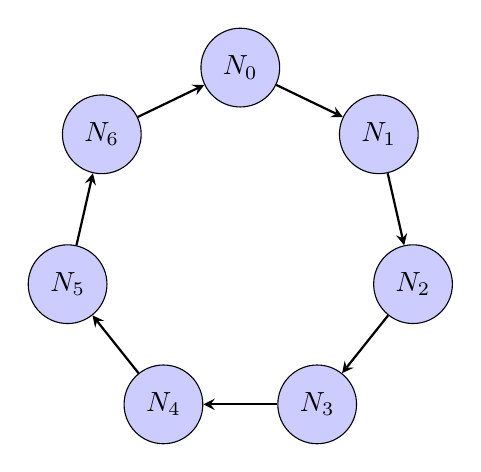
\begin{tikzpicture}[scale=0.9]
    \tikzstyle{node}=[circle, draw, minimum size=1cm, fill=blue!20]

    \foreach \i in {0,...,6} {
        \pgfmathsetmacro{\angle}{90 - \i * 360 / 7}
        \node[node] (n\i) at (\angle:2.5cm) {$N_{\i}$};
    }

    \foreach \i in {0,...,6} {
        \pgfmathtruncatemacro{\j}{mod(\i+1,7)}
        \draw[->, thick, >=stealth] (n\i) -- (n\j);
    }
\end{tikzpicture}
\caption{Krožna topologija s 7 vozlišči. Puščice prikazujejo smer prenosa paketov.}
\label{fig:topology}
\end{figure}

\subsection{Definicija omrežja v NED jeziku}

Omrežje je definirano v datoteki \texttt{ringnetwork.ned}:

\begin{lstlisting}[language=C++, caption={Definicija krožne topologije v NED jeziku}, label=lst:ned]
network circularTopology {
    parameters:
        int numNodes = default(6);
        double datarate @unit(bps) = default(10Mbps);
    submodules:
        node[numNodes]: Node;
    connections allowunconnected:
        for i=0..numNodes-1 {
            node[i].out++ --> DatarateChannel {
                datarate; delay = 1ms;
            } --> node[(i+1) % numNodes].in++;
        }
}
\end{lstlisting}

\subsection{Implementacija vozlišča}

Vozlišče je implementirano v razredu \texttt{Node}, ki deduje od \texttt{cSimpleModule}. Glavne funkcionalnosti vključujejo:

\begin{itemize}
    \item Generiranje paketov z naključnimi ciljnimi vozlišči
    \item Upravljanje čakalne vrste za pakete
    \item Posredovanje paketov naslednjemu vozlišču
    \item Beleženje statistik (zakasnitev, izgubljeni paketi)
\end{itemize}

Ključni del kode za obdelavo paketov:

\begin{lstlisting}[language=C++, caption={Obdelava prejetih paketov}, label=lst:handle]
void Node::handleMessage(cMessage *msg) {
    cPacket *pkt = check_and_cast<cPacket *>(msg);
    int hops = pkt->par("hops");
    int dest = pkt->par("destinationId");

    // Preveri, ce je cilj dosezen
    if (nodeId == dest && hops > 0) {
        simtime_t delay = simTime() - startTime;
        emit(delaySignal, delay);
        delete pkt;
        return;
    }

    // Posreduj naprej
    pkt->par("hops") = hops + 1;
    forwardPacket(pkt);
}
\end{lstlisting}

%%%%%%%%%%%%%%%%%%%%%%%%%%%%%%%%%%%%%%%%%%%%%%%%%%%%%%%%%%%%%%%%%%%%%%%%%%%%%%%
\section{Simulacije in rezultati}
\label{sec:simulacije}

\subsection{Parametri simulacije}

Za analizo zmogljivosti omrežja smo identificirali 5 ključnih parametrov, ki bistveno vplivajo na delovanje:

\begin{table}[H]
\centering
\caption{Parametri simulacije}
\label{tab:parametri}
\begin{tabular}{|l|l|l|}
\hline
\textbf{Parameter} & \textbf{Vrednost} & \textbf{Opis} \\
\hline
numNodes & 7 & Število vozlišč v krogu \\
hopLimit & 10 & Maksimalno število preskokov \\
queueLength & 50 & Dolžina čakalne vrste \\
packetSize & 1 MB & Velikost paketa \\
sendInterval & 1 s (exp.) & Interval pošiljanja \\
\hline
\end{tabular}
\end{table}

\subsection{Konfiguracije obremenitve}

Omrežje smo testirali pri štirih različnih hitrostih prenosa, ki simulirajo različne stopnje obremenitve:

\begin{table}[H]
\centering
\caption{Konfiguracije obremenitve omrežja}
\label{tab:konfiguracije}
\begin{tabular}{|l|l|l|}
\hline
\textbf{Konfiguracija} & \textbf{Hitrost} & \textbf{Obremenitev} \\
\hline
config1 & 1 Mbps & Nadpovprečna (preobremenitev) \\
config2 & 30 Mbps & Normalna \\
config3 & 150 Mbps & Podpovprečna \\
config4 & 500 Mbps & Minimalna \\
\hline
\end{tabular}
\end{table}

\subsection{Analiza povprečnega časa potovanja paketa}

Povprečen čas potovanja paketa od izvornega do ponornega vozlišča (End-to-End Delay) je ključna metrika za oceno zmogljivosti omrežja.

\begin{figure}[H]
\centering
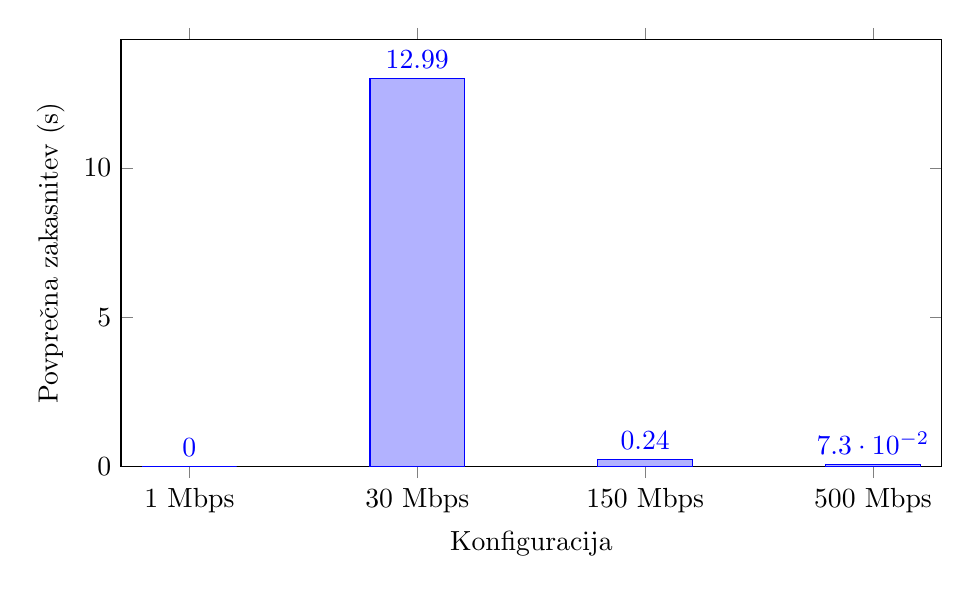
\begin{tikzpicture}
\begin{axis}[
    ybar,
    width=12cm,
    height=7cm,
    ylabel={Povprečna zakasnitev (s)},
    xlabel={Konfiguracija},
    symbolic x coords={1 Mbps, 30 Mbps, 150 Mbps, 500 Mbps},
    xtick=data,
    nodes near coords,
    nodes near coords align={vertical},
    ymin=0,
    bar width=1.2cm,
    fill=blue!60,
]
\addplot coordinates {(1 Mbps, 0) (30 Mbps, 12.99) (150 Mbps, 0.24) (500 Mbps, 0.073)};
\end{axis}
\end{tikzpicture}
\caption{Povprečna zakasnitev paketa pri različnih hitrostih prenosa. Pri 1 Mbps omrežje ni sposobno dostaviti paketov (preobremenitev).}
\label{fig:delay}
\end{figure}

Pri konfiguraciji z 1 Mbps je omrežje popolnoma preobremenjeno -- čakalne vrste se napolnijo in vsi paketi se zavržejo, preden dosežejo cilj. Pri 30 Mbps opazimo povprečno zakasnitev približno 13 sekund, kar kaže na visoko obremenitev. Pri višjih hitrostih (150 Mbps in 500 Mbps) zakasnitev pade pod 1 sekundo.

\subsection{Analiza izgubljenih paketov}

\begin{figure}[H]
\centering
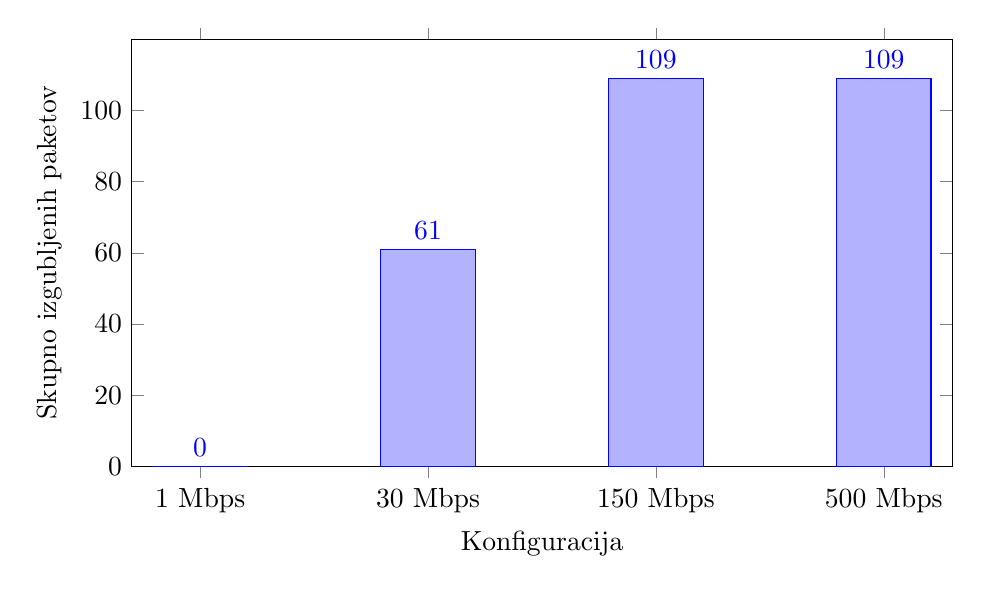
\begin{tikzpicture}
\begin{axis}[
    ybar,
    width=12cm,
    height=7cm,
    ylabel={Skupno izgubljenih paketov},
    xlabel={Konfiguracija},
    symbolic x coords={1 Mbps, 30 Mbps, 150 Mbps, 500 Mbps},
    xtick=data,
    nodes near coords,
    nodes near coords align={vertical},
    ymin=0,
    bar width=1.2cm,
    fill=red!60,
]
\addplot coordinates {(1 Mbps, 0) (30 Mbps, 61) (150 Mbps, 109) (500 Mbps, 109)};
\end{axis}
\end{tikzpicture}
\caption{Število izgubljenih paketov pri različnih konfiguracijah.}
\label{fig:lost}
\end{figure}

Zanimivo opažanje je, da se pri nižji hitrosti (30 Mbps) izgubi manj paketov kot pri višjih hitrostih. To je zato, ker paketi ostanejo v čakalnih vrstah in se počasneje obdelujejo, medtem ko pri višjih hitrostih paketi hitreje krožijo in se vrnejo na izvorno vozlišče (kar šteje kot izguba).

\subsection{Analiza zasedenosti čakalnih vrst}

\begin{figure}[H]
\centering
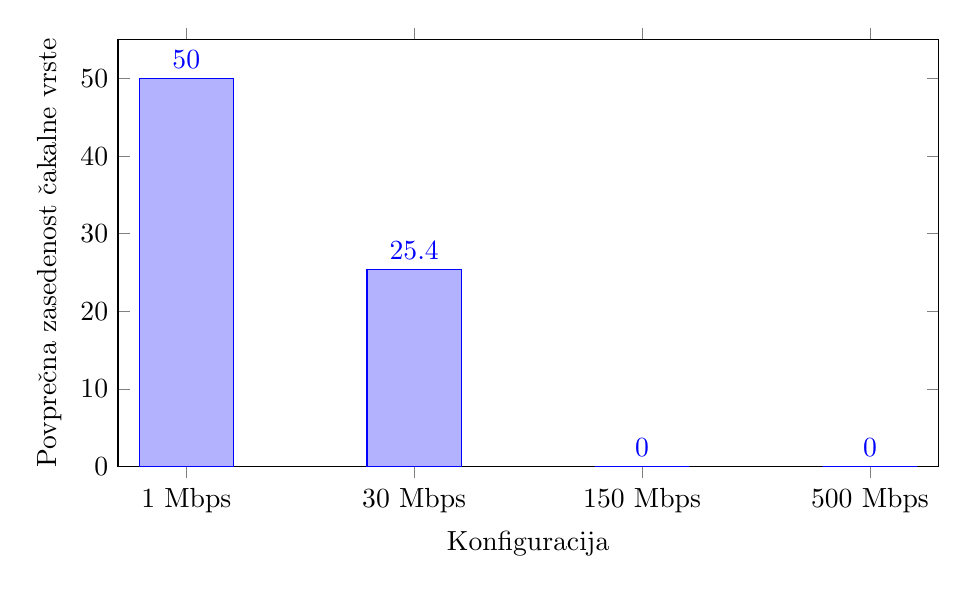
\begin{tikzpicture}
\begin{axis}[
    ybar,
    width=12cm,
    height=7cm,
    ylabel={Povprečna zasedenost čakalne vrste},
    xlabel={Konfiguracija},
    symbolic x coords={1 Mbps, 30 Mbps, 150 Mbps, 500 Mbps},
    xtick=data,
    nodes near coords,
    nodes near coords align={vertical},
    ymin=0,
    ymax=55,
    bar width=1.2cm,
    fill=green!60,
]
\addplot coordinates {(1 Mbps, 50) (30 Mbps, 25.4) (150 Mbps, 0) (500 Mbps, 0)};
\end{axis}
\end{tikzpicture}
\caption{Povprečna zasedenost čakalnih vrst ob koncu simulacije.}
\label{fig:queue}
\end{figure}

Pri 1 Mbps so čakalne vrste popolnoma zasedene (50 elementov -- maksimalna kapaciteta), kar pomeni, da se novi paketi zavržejo. Pri 30 Mbps je povprečna zasedenost približno 25 elementov, kar kaže na zmerno obremenitev. Pri višjih hitrostih so čakalne vrste prazne, kar pomeni, da se paketi prenašajo hitreje, kot se generirajo.

\subsection{Določitev optimalne kapacitete povezav}

Na podlagi rezultatov lahko določimo optimalno kapaciteto povezav za naše omrežje:

\begin{itemize}
    \item \textbf{1 Mbps} -- Popolnoma neustrezno. Omrežje je preobremenjeno in ne more dostaviti paketov.
    \item \textbf{30 Mbps} -- Mejna ustreznost. Visoka zakasnitev (13 s), a paketi se dostavljajo. Čakalne vrste so delno zasedene.
    \item \textbf{150 Mbps} -- Ustrezno. Nizka zakasnitev (0.24 s), prazne čakalne vrste.
    \item \textbf{500 Mbps} -- Prekomerno. Še nižja zakasnitev, a minimalna razlika v primerjavi s 150 Mbps.
\end{itemize}

\textbf{Optimalna kapaciteta}: Glede na razmerje med zmogljivostjo in stroški priporočamo \textbf{150 Mbps} kot optimalno kapaciteto povezav za dano konfiguracijo omrežja (7 vozlišč, 1 MB paketi, 1 s interval pošiljanja).

\subsection{Povzetek rezultatov}

\begin{table}[H]
\centering
\caption{Primerjava rezultatov simulacij}
\label{tab:rezultati}
\begin{tabular}{|l|c|c|c|c|}
\hline
\textbf{Metrika} & \textbf{1 Mbps} & \textbf{30 Mbps} & \textbf{150 Mbps} & \textbf{500 Mbps} \\
\hline
Povp. zakasnitev (s) & 0 & 12.99 & 0.24 & 0.073 \\
Izgubljeni paketi & 0 & 61 & 109 & 109 \\
Zasedenost vrste & 50 & 25.4 & 0 & 0 \\
Stanje omrežja & Blokirano & Obremenjeno & Optimalno & Prosto \\
\hline
\end{tabular}
\end{table}

%%%%%%%%%%%%%%%%%%%%%%%%%%%%%%%%%%%%%%%%%%%%%%%%%%%%%%%%%%%%%%%%%%%%%%%%%%%%%%%
\section{Zaključek}
\label{sec:zakljucek}

V tem seminarju smo uspešno implementirali in analizirali krožno P2P topologijo v orodju OMNeT++. Glavni zaključki so:

\begin{enumerate}
    \item \textbf{Hitrost prenosa} je najpomembnejši parameter, ki vpliva na zmogljivost krožnega omrežja.
    \item Pri prenizki hitrosti (1 Mbps) omrežje postane popolnoma blokirano -- čakalne vrste se napolnijo in paketi se ne morejo dostaviti.
    \item Pri optimalni hitrosti (150 Mbps) dosežemo ravnotežje med nizko zakasnitvijo in učinkovito izrabo virov.
    \item Krožna topologija ima inherentno slabost -- paketi, ki ne dosežejo cilja, krožijo po omrežju in se vrnejo na izvor.
\end{enumerate}

\subsection{Možne nadgradnje}

\begin{itemize}
    \item Implementacija dvosmernega krožnega omrežja za krajše poti
    \item Dodajanje mehanizma za izbiro smeri pošiljanja
    \item Implementacija prioritetnih čakalnih vrst
    \item Analiza vpliva različnega števila vozlišč
\end{itemize}

%%%%%%%%%%%%%%%%%%%%%%%%%%%%%%%%%%%%%%%%%%%%%%%%%%%%%%%%%%%%%%%%%%%%%%%%%%%%%%%
\bibliographystyle{ieeetr}
\bibliography{references}

\end{document}

